\section{おすすめのお土産}
\begin{minipage}{0.45\textwidth}
	\textbf{○萩の月}
	\begin{figure}[H]
		\centering
		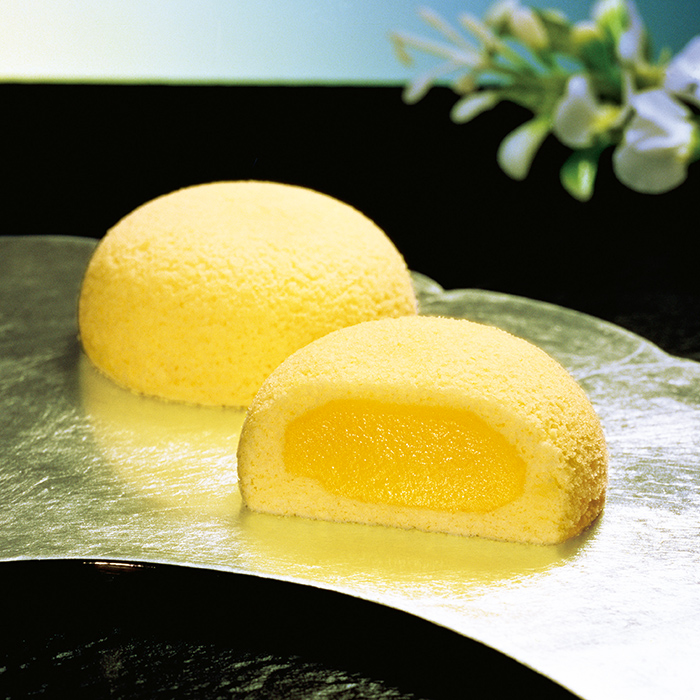
\includegraphics[width=0.6\linewidth]{img/haginotuki}
	\end{figure}
	\begin{center}
		{\scriptsize{菓匠三全 仙台銘菓\\6個入り/1500円}}
	\end{center}
	
	\textbf{○ずんだ餅}
	\begin{figure}[H]
		\centering
		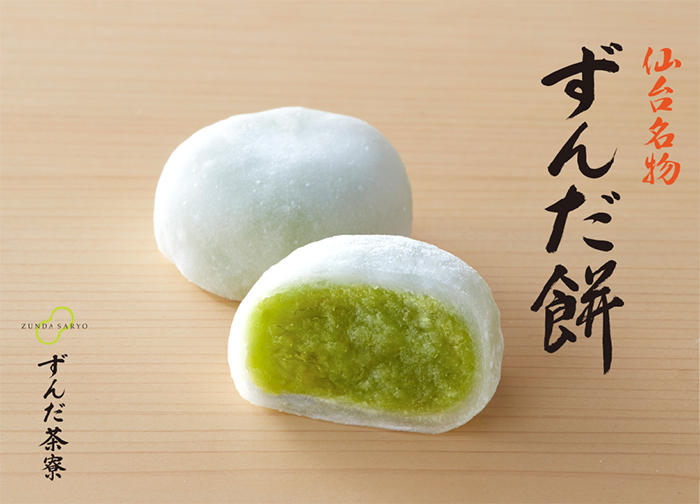
\includegraphics[width=0.65\linewidth]{img/zunda}
	\end{figure}
	\begin{center}
		{\scriptsize{ずんだ茶寮\\8個入り/1080円}}
	\end{center}
	\textbf{○笹かまぼこ}
	\begin{figure}[H]
		\centering
		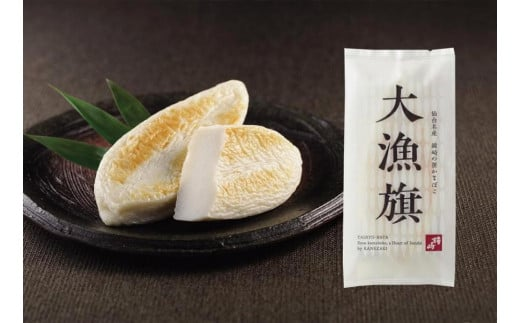
\includegraphics[width=0.7\linewidth]{img/sasakama}
	\end{figure}
	\begin{center}
		{\scriptsize{鐘崎\\330円}}
	\end{center}
	
\end{minipage}
\hspace*{0.5em}
\begin{minipage}{0.45\textwidth}

	\textbf{○霜柱}
	\begin{figure}[H]
		\centering
		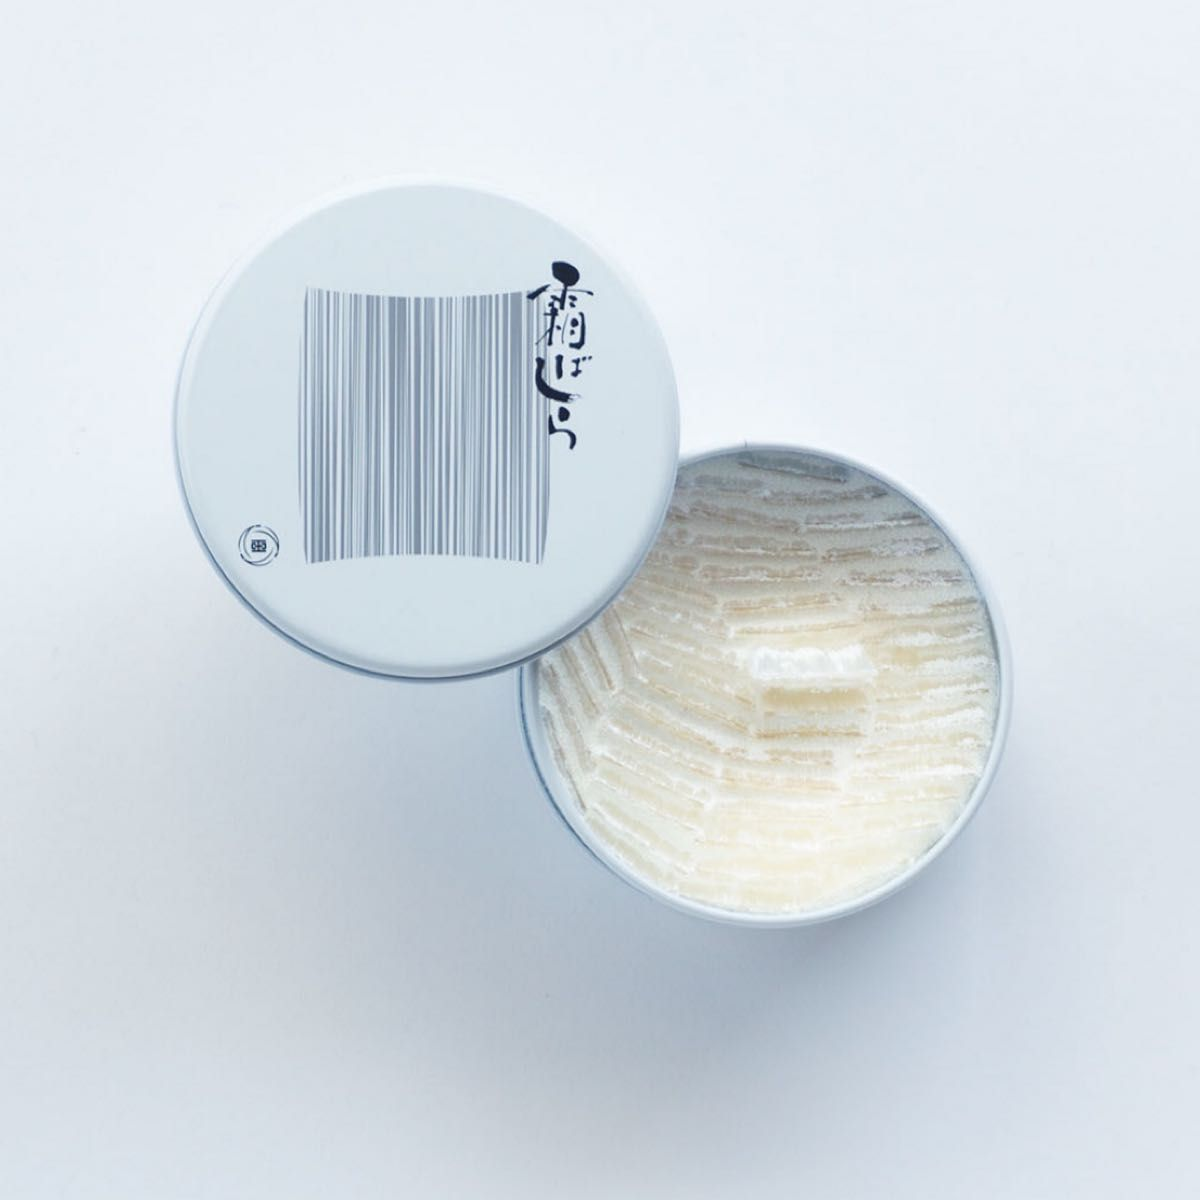
\includegraphics[width=0.5\linewidth]{img/simobashira}
	\end{figure}
	\begin{center}
		{\scriptsize{九重本舗玉澤\\4320円}}
	\end{center}
	\textbf{○仙台ラー油}
	\begin{figure}[H]
		\centering
		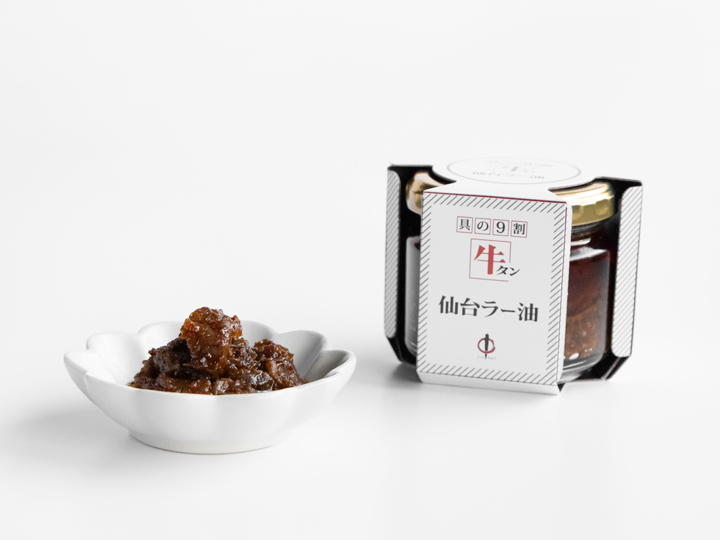
\includegraphics[width=0.6\linewidth]{img/ra-yu}
	\end{figure}
	\begin{center}
		{\scriptsize{牛タン専門店 陣中\\100g/900円}}
	\end{center}
	
	\textbf{○日本酒}
	\begin{figure}[H]
		\centering
		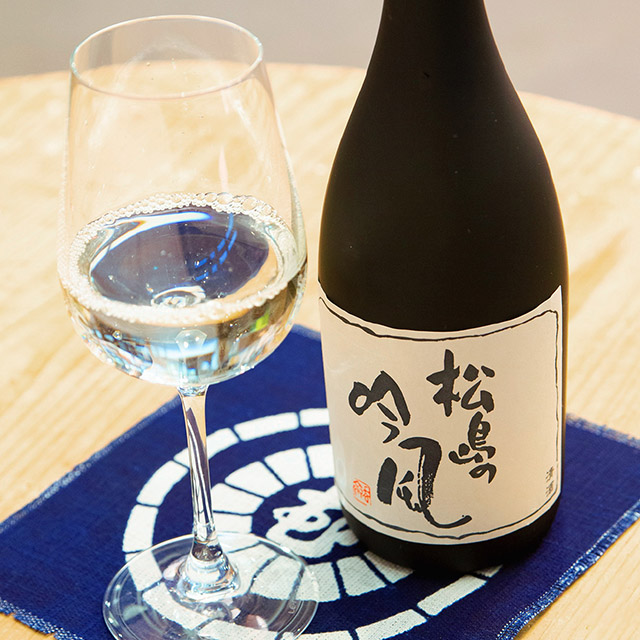
\includegraphics[width=0.6\linewidth]{img/nihonshu}
	\end{figure}
	\begin{center}
		{\scriptsize{むとう屋 仙台駅店\\}}
	\end{center}
\end{minipage}